\section{Management Setup}

\subsection{Jira}
The world of project management offers many different
approaches for which Jira accommodates with an extremely
extensive (and admittedly overwhelming) platform for
configuration.
Although it offers both its own and community-developed
templates, tailoring a standard offering was required to
establish the designed workflow for this project.
Note: Jira uses \enquote{issue} to encapsulate any aspect
of Agile (e.g., epic, theme, user story, bug, etc.)

\begin{figure}[h]
  \centering
  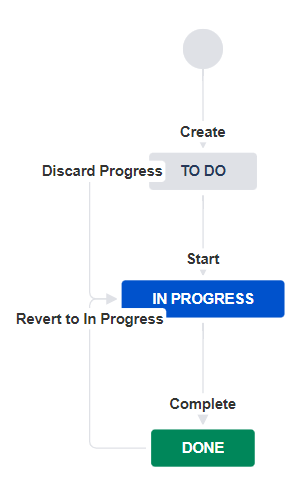
\includegraphics[width=0.4\linewidth]{06
    development/assets/jira workflow.png}
  \caption{Issue status workflow in Jira}
  \label{fig:workflow}
\end{figure}

The first thing required to start work on \projectname{}
was to setup the Jira workflow as per the designed
\hyperref[p:decomp]{task decomposition} and transfer the
epics \& user stories across.

To reduce clutter and optimise readability, the Jira board
is also filtered to only show active epics using a query;
e.g., \lstinline{parentEpic in (RV-1)} only shows issues
within the \enquote{Initiation} epic.
It is also configured to group issues by their user story,
as shown in Figure \ref{fig:kanban}.

\begin{figure}[h]
  \centering
  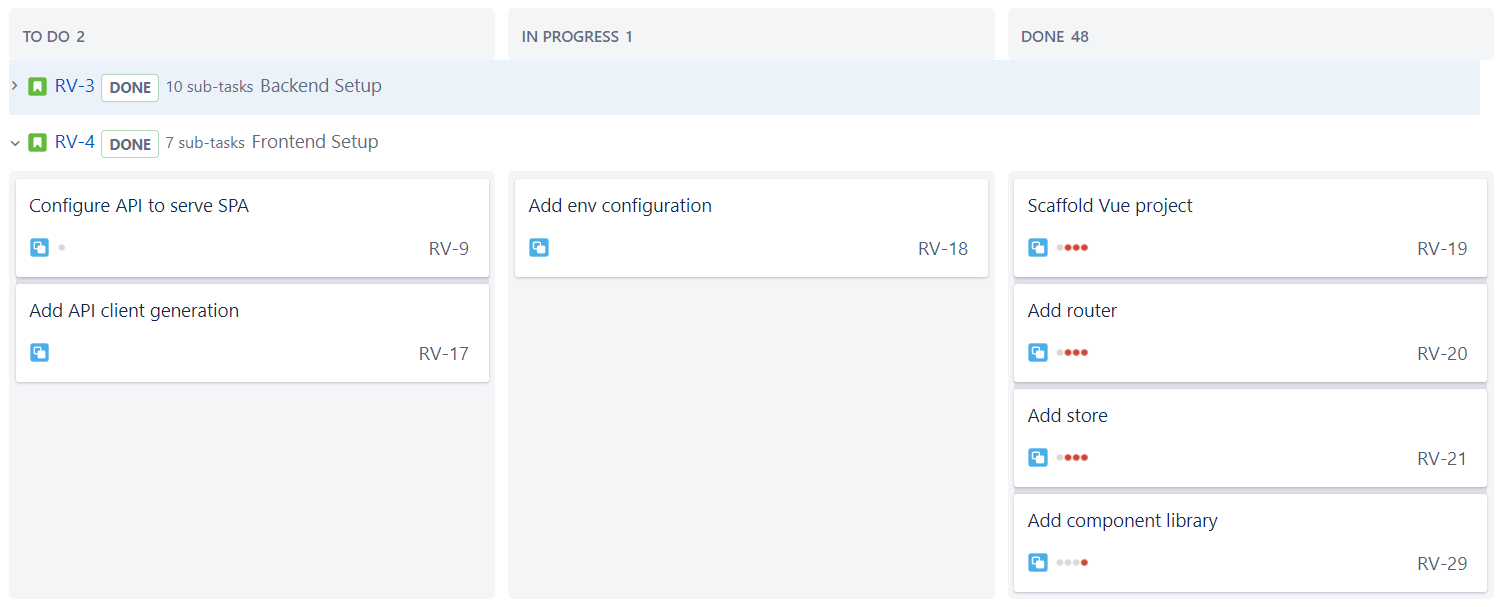
\includegraphics[width=0.9\linewidth]{06
    development/assets/kanban.png}
  \caption{Kanban board in Jira}
  \label{fig:kanban}
\end{figure}

\subsection{Github}
Version control in modern software development is
undisputable necessity --- so I setup a
Github repository. 

The repository is also linked to the Jira board to display
related Github activity for each issue. This is sourced from 
any commit message/branch name/pull request title
containing the issue's ID, as shown in Figure
\ref{fig:jiraGithub};

\begin{figure}[h]
  \centering
  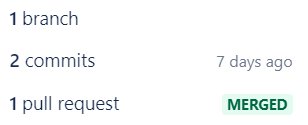
\includegraphics[width=0.6\linewidth]{06
    development/assets/jira github.png}
  \caption{Github integration with Jira}
  \label{fig:jiraGithub}
\end{figure}

The only additional configuration was to restrict the merge
strategy to \enquote{Squash and Merge} which keeps the Git
history tidy. Disabling commits directly to the
\lstinline{master} branch would have also been helpful but
this feature is not available for standard accounts.